%!TEX root = htm.tex
\section{Hybrid transactional memory algorithms}
%
We provide two key observations on this model regarding the interactions of non-committed fast path transactions 
with other transactions. 
Let $E$ be any execution of a HyTM implementation $\mathcal{M}$ in
which a fast-path transaction $T_k$ is either
t-incomplete or aborted. 
Then the sequence of events $E'$ derived by removing all events of $E|k$
from $E$ is an execution  $\mathcal{M}$. Moreover: 
%Then, the following observations are implied by our model.
\begin{observation} 
\label{ob:one}
To every slow-path transaction $T_m \in \ms{txns}(E)$, $E$ is indistinguishable 
from $E'$. 
\end{observation}
%
% \begin{figure*}[t]
% \begin{center}
% 	\subfloat[\label{sfig:ob-01}]{\scalebox{0.5}[0.5]{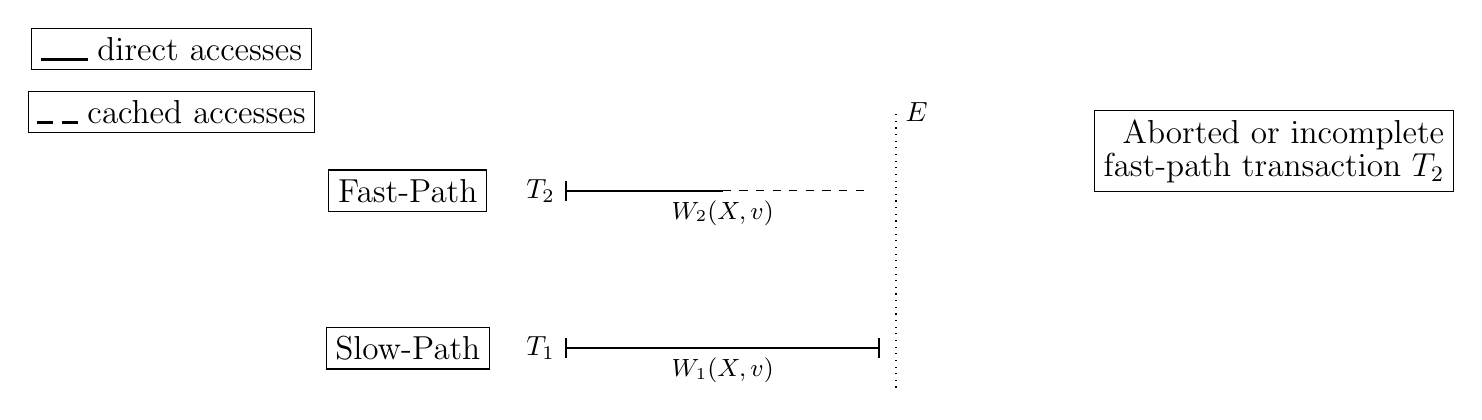
\begin{tikzpicture}
\node (w2) at (10,0) [] {};
\node (w1) at (10,-2) [] {};
\node (w3) at (18,-2) [] {};


\draw (w2) node [below] {\small {$W_2(X,v)$}};

\draw (w1) node [below] {\small {$W_1(X,v)$}};
%\draw (w1) node [below] {\tiny {$T_1$ commits}};

\node[draw,align=left] at (6,0) {{\large Fast-Path}};
\node[draw,align=left] at (6,-2) {{\large Slow-Path}};

\begin{scope}   
\draw [|-,thick] (8,0) node[left] {$T_2$} to (10,0);
\draw [-,dashed] (10,0) to (11.8,0);
\draw [|-|,thick] (8,-2) node[left] {$T_1$} to (12,-2);
\draw [-,dotted] (12.2,-2.5)  to (12.2,1) node[right] {$E$};
\end{scope}
%
\node[draw,align=right] at (17,.5) {\large {Aborted or incomplete}\\ {\large fast-path transaction $T_2$}};
%
\node[draw,align=right] at (3,1.8) {\rule{6mm}{1pt} \large {direct accesses}};
\node[draw,align=right] at (3,1) {\rule{2mm}{1pt} \rule{2mm}{1pt} \large{cached accesses}};

%
\end{tikzpicture}
}}
% 	\hspace{10mm}
% 	\subfloat[\label{sfig:ob-02}]{\scalebox{0.5}[0.5]{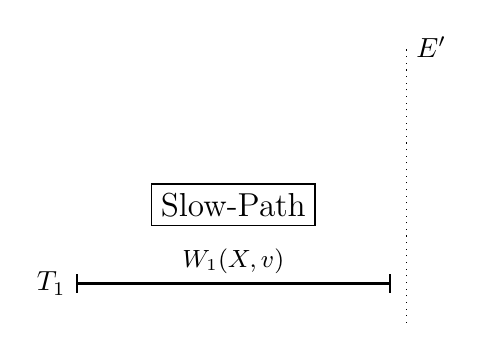
\begin{tikzpicture}

\node (w1) at (11,-2) [] {};


\draw (w1) node [above] {\small {$W_1(X,v)$}};
%\draw (w1) node [below] {\tiny {$T_1$ commits}};

\node[draw,align=left] at (11,-1) {{\large Slow-Path}};

\begin{scope}   
\draw [|-|,thick] (9,-2) node[left] {$T_1$} to (13,-2);
\draw [-,dotted] (13.2,-2.5)  to (13.2,1) node[right] {$E'$};
\end{scope}
%
%
\end{tikzpicture}
}}
% 	 
% \end{center}
% \caption{
% %Executions illustrating
%  %Observation~\ref{ob:one} 
%  \label{fig:ob1}
%  Execution $E$ in Figure~\ref{sfig:ob-01} is indistinguishable
% to $T_1$ from the execution $E'$ in Figure~\ref{sfig:ob-02}}
% \end{figure*}
%
\begin{observation} 
\label{ob:two}
If a fast-path transaction $T_m\in \ms{txns}(E) \setminus \{T_k\}$ does not incur a tracking set abort in $E$, 
then $E$ is indistinguishable to $T_m$ from $E'$.
\end{observation}
%
Intuitively, these observations say that fast-path transactions which are not yet committed are 
invisible to slow-path transactions, and can communicate with other
fast-path transactions only by incurring their tracking-set aborts.
%
%%%%%%%%%%%%%%%%%%%%%%%%%%%%%%%%%%%%%%%%%%%%%%%%%%%%%%%%%%%%%%%%%%%%%
%!TEX root = htm.tex
%%%%%%%%%%%%%%%%%%%%%%%%%%%%%%%%%%%%%%%%%%%%%%%%
\begin{algorithm}[!ht]
\caption{Progressive fast-path and slow-path opaque HyTM implementation; code for transaction $T_k$}
\label{alg:inswrite}
\begin{algorithmic}[1]
  	\begin{multicols}{2}
  	{
  	\footnotesize
	\Part{Shared objects}{
		\State $v_j$, value of each t-object $X_j$ 
		\State $r_{j}$, a versioned lock for each t-object $X_j$
	}\EndPart	
	\Statex
	\Part{Process local objects}{
		\State $\Rset(T_k)$, storing $\{X_j,r_j\}$
		\State $\Wset(T_k)$, storing $\{X_j, v_j\}$
	}\EndPart
	\Statex
	\textbf{Code for fast-path transactions}
	\Statex
	\Part{$\textit{read}_k(X_j)$}\quad\Comment{fast-path}{
		\State $\textit{ov}_j := \Read(v_j)$ \Comment{cached read} \label{line:lin1}
		\State $\textit{or}_j := \Read(r_j)$ \Comment{uncached read}
		\If{$\textit{or}_j$ $\mathrel{\&}1$}  \label{line:hread}
			\Return $A_k$ \EndReturn
		\EndIf
		
		\Return $\textit{ov}_j$ \EndReturn
		
   	 }\EndPart
	\Statex
	%\Comment{What is the best strategy to buffer writes?}
	\Part{$\textit{write}_k(X_j,v)$}{\quad\Comment{fast-path}
		\State $\textit{or}_j := \Read(r_j)$ \Comment{cached read}
		\If{$\textit{or}_j$ $\mathrel{\&} 1$}  		
			\Return $A_k$ \EndReturn
		\EndIf
		
		\State $\Write(r_j,\textit{or}_j+2)$ \Comment{uncached write}
		\State $\Write(v_j,v)$ \Comment{uncached write} 
		\Return $\ok$ \EndReturn
		
   	}\EndPart
	\Statex
	
	\Part{$\textit{tryC}_k$()}{\quad\Comment{fast-path}
		\State $\ms{commit-cache}_i$ \label{line:lin3} \Comment{returns $C_k$ or $A_k$}
  	 }\EndPart
  	 
  	 \Statex
  	\Part{Function: $\lit{release}(Q)$}{
  		\ForAll{$X_j \in Q$}	
 			\State $r_j.\lit{write}(or_j+1)$ \label{line:rel1}	
		\EndFor
		
	}\EndPart
 	\Statex
	\Part{Function: $\lit{acquire}(Q)$}{
  		\ForAll{$X_j \in Q$}	
 			\If{ $r_j.\lit{setV}()$} \label{line:acq1}
			  \State $\ms{Lset}(T_k):=\ms{Lset}(T_k)\cup \{X_j\}$
			  \Return $\true$ \EndReturn
			\EndIf
			\State $\lit{release}(\ms{Lset}(T_k))$
			\Return $\false$ \EndReturn
		\EndFor
		
	}\EndPart
	\Statex
	\Statex \Comment{Implement using LL/SC on Power8}
	\Part{Function: $\lit{setV}()$}{
% 		\State $\ms{success} \gets \lit{false}$
% 		
% 		\While{($\neg \ms{success}$)} \Comment {spin until we get the lock}
		%\State $\ms{or}_j \gets$ $r_j.\Read()$ $\mathrel{\&}1111...1110$
		\If{$r_j$.CAS($or_j$, $or_j+1$)} 
		  \Return $\false$  \EndReturn
		\EndIf
		\Return $\true$ \EndReturn
	}\EndPart
  	 
  	 \newpage
	\textbf{Code for slow-path transactions}
	\Statex
	\Part{\Read$_k(X_j)$}\quad\Comment{slow-path}{
		  \If{$X_j\in \Wset(T_k)$}
		    \Return $\Wset(T_k).\lit{locate}(X_j)$ \EndReturn
		  \Else
		  
		  \State $\textit{or}_j := \Read(r_j)$ \label{line:readorec}
		  \State $\textit{ov}_j := \Read(v_j)$ \label{line:read2}
		  \State $\Rset(T_k) := \Rset(T_k)\cup\{X_j,or_j\}$ \label{line:rset}
		  \If{$\textit{or}_j$ $\mathrel{\&} 1$} \label{line:abort0}	
			\Return $A_k$ \EndReturn
		  \EndIf
		 
		  \If{$\neg \lit{validate}()$} \label{line:valid}
			\Return $A_k$ \EndReturn
		  \EndIf
		  \EndIf
		  \Return $\textit{ov}_j$ \EndReturn
		
   	 }\EndPart
	\Statex
	\Part{\Write$_k(X_j,v)$}\quad\Comment{slow-path}{
		
			\State $\textit{or}_j := \Read(r_j)$
			\State $\textit{nv}_j := v$
			\If{$\textit{or}_j$ $\mathrel{\&} 1$}	
			\Return $A_k$ \EndReturn
			\EndIf
			\State $\Wset(T_k) := \Wset(T_k)\cup\{X_j,\textit{nv}_j\}$
			\Return $\ok$ \EndReturn
		
   	}\EndPart
	\Statex
	
	%\Statex	
	\Part{\TryC$_k$()}\quad\Comment{slow-path}{
		\If{$\Wset(T_k)= \emptyset$}
			\Return $C_k$ \EndReturn \label{line:return}
		\EndIf
		\If{$\lit{acquire}(\Wset(T_k))$}	\label{line:acq}
		
		\If{$\neq \lit{validate}()$} \label{line:abort3}
			\State $\lit{release}( \ms{Wset}(T_k))$ 
			\Return $A_k$ \EndReturn
		\EndIf
		\ForAll{$X_j \in \Wset(T_k)$}
	 		\State  $v_j.\lit{write}(\textit{nv}_j)$ \label{line:write}
			 
	 	\EndFor	
		  
		\State $\lit{release}(\Wset(T_k))$   \label{line:rel}	
   		\Return $C_k$ \EndReturn
   		\Else
		  \Return $A_k$ \EndReturn
		  \EndIf
   	 }\EndPart		
	 
 	
	\Statex
	\Part{Function: $\lit{validate}()$}{\quad\Comment{Validate slow-path reading transactions}
		\If{$\exists X_j \in Rset(T_k)$;$X_j \not\in \Wset(T_k)$:$(\textit{or}_j\neq \Read(r_j))$} \label{line:valid}
			\Return $\false$ \EndReturn
		  \EndIf
		 \Return $\true$ \EndReturn
	}\EndPart
		
  	 }
	\end{multicols}
  \end{algorithmic}
\end{algorithm}
%%%%%%%%%%%%%%%%%%%%%%%%%%%%%%%%%%%%%%%%%%%%%%%%
\begin{figure*}[!h]
      
     \scalebox{.9}[.9]{
     \begin{tabularx}{\textwidth}{c|c|c|c|c}
%	\hline
	~~~~~ & Algorithm~\ref{alg:inswrite} & Algorithm~\ref{alg:inswrite2} & TLE & HybridNorec\\ \hline
	Instrumentation in fast-path reads & per-read & none & none & none \\ \hline
	Instrumentation in fast-path writes & per-write & per-write & constant & none \\ \hline
	Validation in slow-path reads & $\Omega(|Rset|)$ & $\Omega(|Rset|)$ & None & $\Omega(|Rset|)$ only if concurrency \\ \hline
	h/w-s/f concurrency & prog. & prog. for slow-path readers & zero & not prog., but small contention window \\ \hline
	Uncached accesses inside fast-path & yes & yes & no & yes \\ \hline
	opacity & yes & yes & Yes & Yes 
	%    \hline
   \end{tabularx}
\caption{Table}\label{fig:main}    
}
\end{figure*}
%%%%%%%%%%%%%%%%%%%%%%%%%%%%%%%%%%%%%%%%%%%%%%%%%%%
\subsection{Instrumentation-optimal progressive HyTMs }
\label{sec:hytm1}
%
For every t-object $X_j$, our implementation maintains a base object $v_j\in \mathbb{D}$ that stores the value of $X_j$
and a \emph{sequence lock} $r_{j}$. The sequence lock is an unsigned integer whose LSB bit stores the \emph{locked} state.
Specifically, we say that process $p_i$ \emph{holds a lock on $X_j$ after an execution $E$} if
$\textit{or}_j$ $\mathrel{\&} 1=1$ after $E$, where $\textit{or}_j$ is the value of $r_j$ after $E$.

\vspace{1mm}\noindent\textit{Fast-path transactions:}
For a fast-path transaction $T_k$ executed by process $p_i$, the $\Read_k(X_j)$ implementation first reads $r_j$ (uncached)
and returns $A_k$ if some other process $p_j$ holds a lock on $X_j$.
Otherwise, it returns the value of $X_j$.
Updating fast-path transactions 
As with $\Read_k(X_j)$, the $\Write (X_j,v)$ implementation returns $A_k$ if some other process $p_j$ holds a lock on $X_j$.
Process $p_i$ then increments the value of $r_j$ by $2$ via a direct access and stores the cached state of $X_j$ along with its value $v$.
If the cache has not been invalidated, $p_i$ updates the shared memory
during $\TryC_k$ by invoking the $\ms{commit-cache}$ primitive.

\vspace{1mm}\noindent\textit{Slow-path read-only transactions:}
Any $\Read_k(X_j)$ invoked by a slow-path transaction first reads the value of the object from $v_j$, 
checks if $r_j$ is se, adds $r_j$ to $\Rset(T_k)$
and then performs \emph{validation} on its entire read set to check if any of them have been modified. 
If either of these conditions is true,
the transaction returns $A_k$. Otherwise, it returns the value of $X_j$. 
Validation of the read set is performed by re-reading the values of the sequence lock entires stored in $\Rset(T_k)$.
%A read-only transaction simply returns $C_k$ during the tryCommit.

\vspace{1mm}\noindent\textit{Slow-path updating transactions:}
% The $\Write_k(X,v)$ implementation of a slow-path transaction stores
% $v$ and the current value of $X_j$ locally, 
% deferring the actual update in shared memory to tryCommit. 
An updating slow-path transaction $T_k$ attempts to obtain exclusive write access to its 
entire write set by performing \emph{compare-and-set} (\emph{cas})
primitive that checks if the value of $r_j$, for each $X_j\in \Wset(T_k)$, is unchanged since last reading it during $\Write_k(X.v)$
If all the locks on the write set were acquired successfully, $T_k$ performs validation of the read set and returns $C_k$ if successful, else $p_i$ aborts the transaction.

\vspace{1mm}\noindent\textit{Non-cached accesses inside fast-path:}
As indicated in the pseudocode of Algorithm~\ref{alg:inswrite}, some accesses may be performed uncached (as allowed
in IBM Power 8) and the resulting implementation would still be opaque. 
% We can now prove the following theorem:
% %
% \begin{theorem}
% \label{th:inswrite}
% Algorithm~\ref{alg:inswrite} implements an opaque HyTM that provides invisible reads, progressiveness
% such that in its every execution $E$, every fast-path transaction $T\in \ms{txns}(E)$
% accesses $m=|\Dset(T_k)|$ distinct metadata base objects.
% \end{theorem}
%

\vspace{1mm}\noindent\textbf{Instrumentation-optimal HyTMs that are progressive only for a subset of transactions.}
Algorithm~\ref{alg:inswrite2} does not incur the linear instrumentation cost
on the fast-path reading transactions (as in Algorithm~\ref{alg:inswrite}, but provides progressiveness only
for slow-path reading transactions.
%
%%%%%%%%%%%%%%%%%%%%%%%%%%%%
\begin{algorithm*}[!ht]
\caption{Opaque HyTM implementation with sequential slow-path and progressive fast-path TM-progress; code for $T_k$ by process $p_i$}
\label{alg:inswrite2}
\begin{algorithmic}[1]
  	\begin{multicols}{2}
  	{
  	\footnotesize
	\Part{Shared objects}{
		\State $v_j \in \mathbb{D}$, for each t-object $X_j$ 
		%\Statex ~~~~~allows reads, writes
		\State $r_{j}$, sequence lock for each t-object $X_j$
		\State $L$, global single-bit lock
		%\Statex ~~~~~allows reads, writes 
		%\State implemented from reads and writes
		%\State $L$, multi-trylock
	}\EndPart	
% 	\Statex
% 	\Part{Process local objects}{
% 		\State $\Rset(T_k)$, storing $\{X_j,r_j\}$
% 		\State $\Wset(T_k)$, storing $\{X_j, v_j\}$
% 	}\EndPart
	\Statex
	\textbf{Code for fast-path transactions}	
	\Statex
	\Part{$\textit{start}_k()$}{
		
		\State $l \gets \Read(\ms{L})$ \Comment{cached read} 
		\If{$\ms{l} \mathrel{\&} 1\neq 0$}
			    \Return $A_k$ \EndReturn
		\EndIf
		
	}\EndPart
	\Statex
	%\Comment{In general, would it better to buffer writes in tryC?}
	\Part{$\textit{read}_k(X_j)$}{\quad\Comment{fast-path}
		
		\State $\textit{ov}_j := v_j.\Read()$ \Comment{cached read} 
		
		\Return $\textit{ov}_j$ \EndReturn
		
   	 }\EndPart
	\Statex
	\Part{$\textit{write}_k(X_j,v)$}{\quad\Comment{fast-path}
	
	\State $\underline{\textit{or}_j := \Read(r_j)}$ \Comment{uncached read}
	\State $\underline{r_j.\Write({or}_j+2)}$ \Comment{uncached write}
	\State $v_j.\Write(v)$ \Comment{cached write}
	\Return $\ok$ \EndReturn
		
   	}\EndPart
	\Statex
	
	%\Statex	
	\Part{$\textit{tryC}_k$()}{\quad\Comment{fast-path}
		%\Return $C_k$ \EndReturn
		\State $\ms{commit-cache}_i$ \Comment{returns $C_k$}
		
   		
   	 }\EndPart		
   	 \Statex
	\Statex
	\textbf{Code for slow-path transactions}
	\Statex
	\Part{$\textit{start}_k()$}{
		
		\State $l \gets \Read(\ms{L})$
				
	}\EndPart
	\Statex
	\Part{\Read$_k(X_j)$}\quad\Comment{slow-path}{
		  \If{$X_j\in \Wset(T_k)$}
		    \Return $\Wset(T_k).\lit{locate}(X_j)$ \EndReturn
		  \Else
		  \State $\textit{ov}_j := \Read(v_j)$ 
		  \State $\textit{or}_j := \Read(r_j)$ 
		  \State $\Rset(T_k) := \Rset(T_k)\cup\{X_j,or_j\}$ 
		  \If{$\textit{or}_j$ $\mathrel{\&} 1$}  	
			\Return $A_k$ \EndReturn
		  \EndIf
		  \If{$\neg \lit{validate}()$}
			\Return $A_k$ \EndReturn
		  \EndIf
		  \EndIf
		  \Return $\textit{ov}_j$ \EndReturn
		
   	 }\EndPart
   	\newpage
	\Part{\Write$_k(X_j,v)$}\quad\Comment{slow-path}{
		
			\State $\textit{nv}_j := v$
			\State $\Wset(T_k) := \Wset(T_k)\cup\{X_j,nv_j\}$
			\Return $\ok$ \EndReturn
		
   	}\EndPart
	\Statex
	
	%\Statex	
	\Part{\TryC$_k$()}\quad\Comment{slow-path}{
		\If{$\Wset(T_k)= \emptyset$}
			\Return $C_k$ \EndReturn 
		\EndIf
				
		\While {$\neg flag$}
		  \State $flag \gets L.\lit{cas}(0,1)$
		\EndWhile
		\ForAll{$X_j \in Q$}	
			\State $or_j\gets r_j.\lit{read}()$ 
			 		
		\EndFor
		\Comment{First read, then write all: single barrier}
		\ForAll{$X_j \in Q$}	
			\State $r_j.\lit{write}(or_j + 1)$ 
			 		
		\EndFor
		\If{$\lit{validate}()$}
			\State \textbf{goto} Line~\ref{line:release}
			
		\EndIf
		
		\ForAll{$X_j \in \Wset(T_k)$}
	 		 \State  $v_j.\lit{write}(\textit{nv}_j)$
			 
			 
	 	\EndFor		
		
  		\ForAll{$X_j \in \Wset(T_k)$}	\label{line:release}
 			\State $r_j.\lit{write}(or_j + 1)$ 
		\EndFor
		
		\State $L.\lit{write}(1)$
   		\Return $C_k$ \EndReturn
   	 }\EndPart		
	\Statex
	\Part{Function: $\lit{validate}()$}{
		
		\If{$\exists X_j \in Rset(T_k)$:$(\textit{or}_j\neq \Read(r_j))$}
			\Return $\false$ \EndReturn
		  \EndIf
		
		 \Return $\true$ \EndReturn
	}\EndPart
	
% 	
	}
	\end{multicols}
  \end{algorithmic}
\end{algorithm*}

%%%%%%%%%%%%%%%%%%%%%%%%%%%%%%%%%%%%%%%%%%%%%%%%
%
\subsection{Minimizing the cost for incremental validation in opaque HyTMs}
\label{sec:middlepath}
%
%
Observe that the lower bound in Theorem~\ref{th:impossibility} assumes progressiveness for both slow-path and fast-path transactions
along with opacity and invisible reads.
In this section, we suggest algorithmic ideas for cirvumventing the lower bound or minimizing the cost incurred
by implementations due to incremental validation. Figure~\ref{fig:main} summarizes the complexity costs
associated with the HyTM algorithms considered in this paper.

\vspace{1mm}\noindent\textbf{Sacrificing progressiveness and minimizing contention window.}
%
\emph{Hybrid NOrec}~\cite{hybridnorec} is a HyTM implementation that does not satisfy progressiveness
(unlike its STM counterpart NOrec), but mitigates
the step-complexity cost on slow-path transactions by performing incremental validation 
during a transactional read \emph{iff} 
the shared memory has changed since the start of the transaction.
Conceptually, hybrid NOrec uses a global sequence lock gsl that is incremented 
at the start and end of each transaction's commit procedure.
Readers can use the value of gsl to determine whether shared memory has changed between two configurations.
Unfortunately, with this approach, two fast path transactions will always conflict on the gsl if their 
commit procedures are concurrent.
To reduce the contention window for fast path transactions, the gsl is actually implemented as two separate locks.
A slow path transaction locks both esl and gsl while it is committing.
Instead of incrementing gsl, a fast path transaction checks if esl is locked and aborts if it is.
Then, at the end of the fast path transaction's commit procedure, 
it increments gsl twice (quickly locking and releasing it and immediately commits in hardware), thus, the 
window for fast path transactions to content on gsl is very small.

\vspace{1mm}\noindent\textbf{Employing an uninstrumented fast fast-path.}
Note that ideally we would like to execute all transactions inside hardware with minimal instrumentation.
We now describe how every transaction may first be executed in a ``fast'' fast-path with almost no instrumentation
and if unsuccessful, may be re-attempted in the fast-path and subsequently in slow-path.
Specifically, Algorithm~\ref{alg:middle} describes a generic transformation for any opaque HyTM $\mathcal{M}$ to an opaque
HyTM $\mathcal{M}'$ by employing a shared \emph{fetch-and-add} metadata $F$ that slow-path updating transactions
increment (and resp. decrement) at the start (and resp. end). The fast fast-path checks first checks if $F$ is $0$
and if not, aborts the transaction; otherwise the transaction is continued as an uninstrumented hardware transaction.
Since there is no concurrency between fast fast-path and slow-path, opacity is immediate.
%
%
\begin{algorithm*}[!h]
\caption*{\textbf{Algorithm 1+} Transformation for opaque HyTM $\mathcal{M}$ to include a fast fast-path; code for $T_k$ by process $p_i$}
\label{alg:middle}
\vspace{-1mm}
\noindent\lstset{style=customc}
\begin{minipage}{0.49\textwidth}
\begin{lstlisting}[frame=none,firstnumber=1,mathescape=true]
//\textbf{Shared objects}
    F, fetch-and-increment object
    
//\textbf{Code for slow-path transactions}
tryC$_k$()
    if $\Wset(T_k)= \emptyset$ then
	return C$_k$  
    $F.\lit{fetch-add}(1)$
    //\textbf{Invoke updating slow-path tryC$_k$(); let $r_k$ be the response}
    $F.\lit{fetch-add}(-1)$
    return r$_k$ 
\end{lstlisting}
\end{minipage}
\begin{minipage}{0.49\textwidth}
\begin{lstlisting}[frame=none,firstnumber=last,mathescape=true]
//\textbf{Code for fast fast-path transactions}
start$_k$()
    if F $\neq 0$ then //\medcom cached read
	return A$_k$

read$_k$(X$_j$)
    ov$_j$ := v$_j$ //\medcom cached read 
    return ov$_j$
		
write$_k$(X$_j$,v)
    v$_j$:=v  //\medcom cached write
    return ok

tryC$_k$()
    commit-cache$_i$ //\medcom returns C$_k$ or A$_k$
\end{lstlisting}
\end{minipage}
\end{algorithm*}



% \begin{algorithmic}[1]
%   	\begin{multicols}{2}
%   	{
%   	\footnotesize
% 	\Part{Shared objects}{
% 		%\State $v_j$, for each t-object $X_j$ 
% 		\State $F$, fetch-and-increment object
% 		
% 	}\EndPart	
%  	\Statex
%  	\Statex
%  	\textbf{Code for slow-path transactions}
% 	\Statex
% 	\Part{$\textit{tryC}_k$()}{\quad\Comment{slow-path}
% 		\If{$\Wset(T_k)= \emptyset$}
% 			\Return $C_k$ \EndReturn 
% 		\EndIf
% 		\State $F.\lit{fetch-add}(1)$
% 		\State \textbf{Invoke updating slow-path $\TryC_k()$; let $r_k$ be the response}
% 		
% 		\State $F.\lit{fetch-add}(-1)$
% 		\Return $r_k$ \EndReturn
%    		
%    	 }\EndPart		
% 	\newpage
% 	\textbf{Code for fast fast-path transactions}	
% 	\Statex
% 	\Part{$\textit{start}_k()$}{
% 		
% 		\If{$\Read(\ms{F}) \neq 0$} \Comment{cached read}
% 		  \Return $A_k$ \EndReturn
% 		\EndIf
% 		
% 	}\EndPart
% 	\Statex
% 	%\Comment{In general, would it better to buffer writes in tryC?}
% 	\Part{$\textit{read}_k(X_j)$}{\quad\Comment{fast fast-path}
% 		
% 		\State $\textit{ov}_j := v_j.\Read()$ \Comment{cached read} 
% 		
% 		\Return $\textit{ov}_j$ \EndReturn
% 		
%    	 }\EndPart
% 	\Statex
% 	\Part{$\textit{write}_k(X_j,v)$}{\quad\Comment{fast fast-path}
% 	
% 	\State $v_j.\Write(v)$ \Comment{cached write}
% 	\Return $\ok$ \EndReturn
% 		
%    	}\EndPart
% 	\Statex
% 	
% 	%\Statex	
% 	\Part{$\textit{tryC}_k$()}{\quad\Comment{fast fast-path}
% 		%\Return $C_k$ \EndReturn
% 		\State $\ms{commit-cache}_i$ \Comment{returns $C_k$ or $A_k$}
% 		
%    		
%    	 }\EndPart		
%    	   	
% 	
% 	}
% 	\end{multicols}
%   \end{algorithmic}
% \end{algorithm*}

%%%%%%%%%%%%%%%%%%%%%%%%%%%%%%%%%%%%%%%%%%%%
%
%
